To evaluate our solution we have performed experiments on a collection of 100 different proteins.
The average protein length is 78.12 amino acids spanning between 11 and 415.
The total running time of our fitting algorithm is around 2 minutes for the protein of length 415 on a 1.86GHz CPU.
There should be ample room for code optimizations as this has not been the focus of the project.

\section{Backbone fitting}
When fitting a protein to a given \Ca-trace we are interested in minimizing the RMSD while avoiding collisions.
In this section we will only consider the RMSD as the evaluation of our collision avoidance method  is delayed until Section \ref{sec:evaluation_handling_side-chains}. 

Typically we are able to reach an RMSD less than 0.2 Å with our backbone fitting algorithm (Algorithm \ref{alg:ccd}).
This is considered satisfactory by the algorithms group at our department.
% We will wait until Sectionwill not consider the collision when evaluating the backbone fitting algorithm.
%In this experiment we have let our algorithm perform the same amount of work for different window sizes (ie. for small $w$ the number of window repetitions is large and vice versa).
\newpage\vspace*{-15mm}
\subsection{Choice of window size}
As our fitting method performs CCD on a window within the backbone it is interesting to investigate the effect when varying the window size $w$.
Figure \ref{fig:rmsd_convergence} shows the RMSD for four different window sizes $w$ as we repeat the fitting algorithm one to ten times.
\begin{figure}
	\centering
	\hspace*{-3.5mm}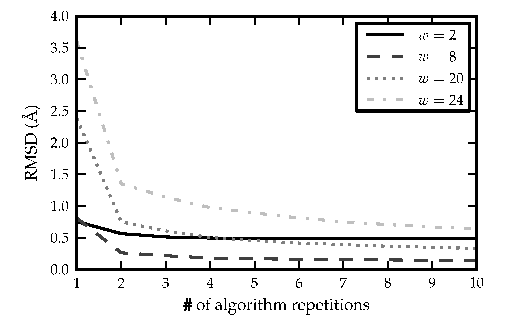
\includegraphics[width=1.1\columnwidth]{figures/plot_rmsd_convergence}
	\caption{RMSD as the fitting progresses for different choices of window size $w$.}
	\label{fig:rmsd_convergence}
\end{figure}
After the first iteration we see that a small window size allows the fitting method to be flexible and reach a low RMSD quickly.
However, if $w$ is too small, the fitting does not improve as we repeat the algorithm.
This is because the chosen angles from a small window are too greedy and find local solutions that lead to an unfavorable global backbone conformation.
On the other hand if $w$ is too large, we see that the RMSD improves in each iteration but requires many iterations to reach a low RMSD.
The problem is caused by the end-effector becoming too large such that there is no clear direction towards the target since all the elements of the end-effector must go in different directions to reach their separate targets.
This results in small angular changes in each step of the CCD method and a slow RMSD convergence.
Thus, in determining the window size we must strike a balance between small and flexible to get fast convergence and large with the ability to better capture the optimal global solution.
To better illustrate the relationship between RMSD and $w$, the RMSD after 10 repetitions is plotted as a function of $w$ in Figure \ref{fig:rmsd_windowsize}.
We see that the optimal window size is between 5 and 12 amino acids.
\begin{figure}
	\centering
	\hspace*{-3.5mm}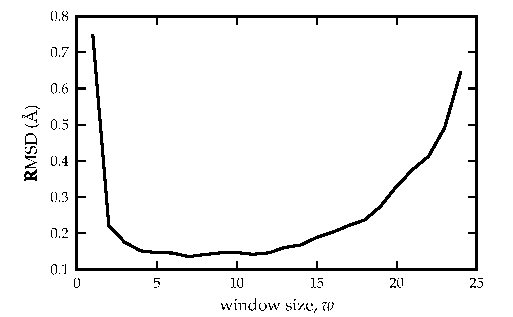
\includegraphics[width=1.1\columnwidth]{figures/plot_rmsd}
	\caption{RMSD as a function of the window size.}
	\label{fig:rmsd_windowsize}
\end{figure}



\subsection{Ramachandran plot}
To check if our fitted backbone structure contains realistic pairs of $\phi$ and $\psi$ angles we can inspect the resulting Ramachandran plots.
Figure \ref{fig:eval_ramachandran} shows two Ramachandran plots of a protein and our fitted backbone version of the same protein.
In the fitted protein the dense region (the $\alpha$-helix region) resembles the original.
There is also a very slight resemblance in the upper left corner (the $\beta$-sheet region).
More problematic, we see for the fitted protein that a large part of the angle sets are spread out in the Ramachandran space.
This indicates that we are likely to have unrealistic angle sets since these do not occur in the original backbone nor in Figure \ref{fig:ramachandran}.

\begin{figure*}
	\centering
	\hspace{1cm}\subbottom[]{\hspace{0.2cm}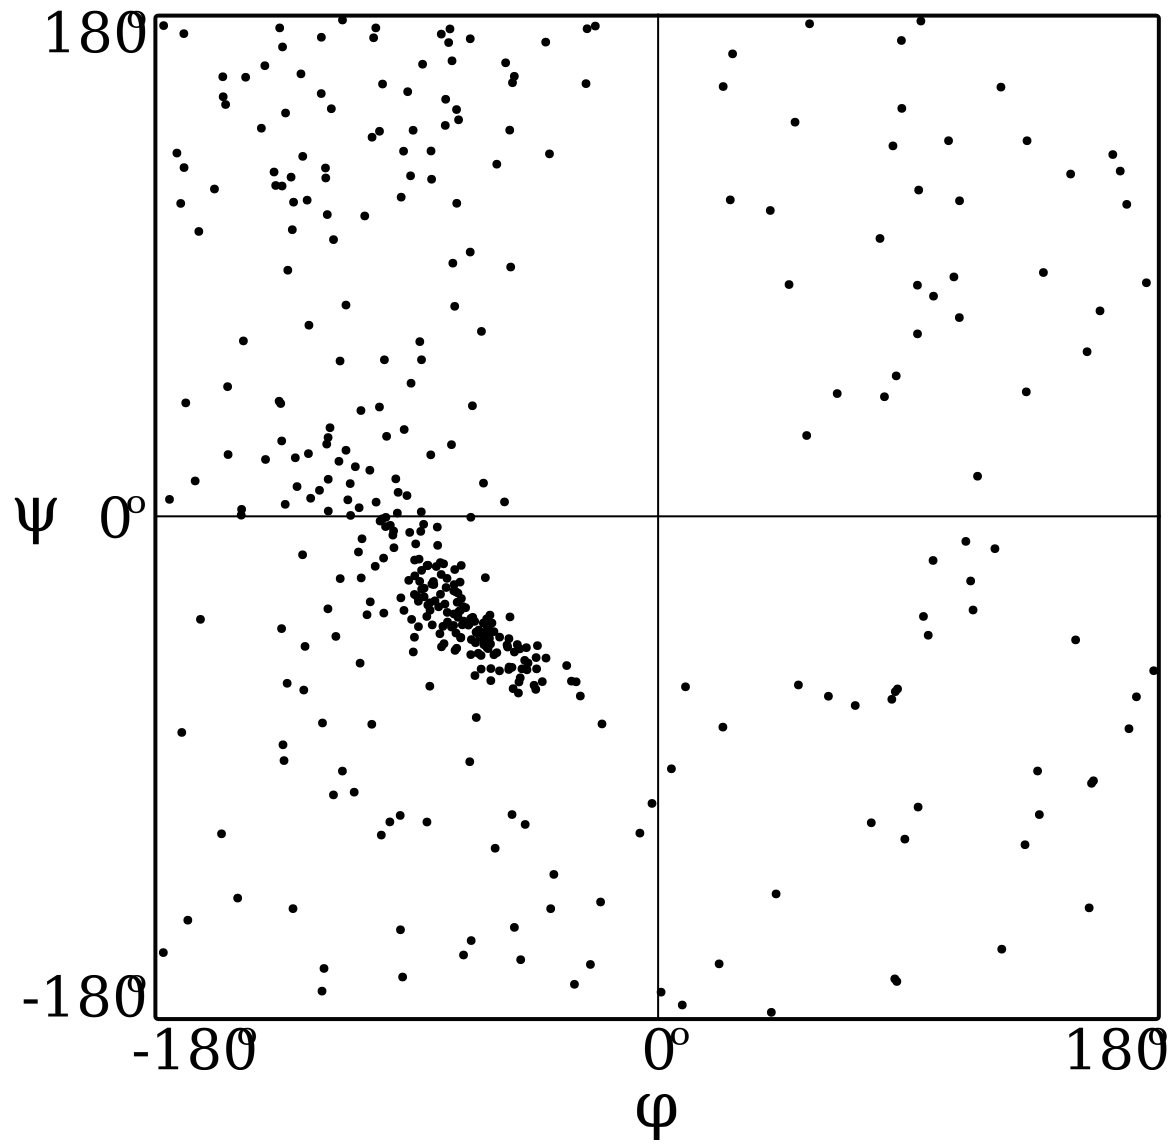
\includegraphics[width=0.75\columnwidth]{figures/plot_ramachandran_orig}\hspace{1cm} \label{fig:eval_ramachandran_orig}}\hspace{0.5cm}\subbottom[]{\label{fig:eval_ramachandran_fitted}\hspace{0.3cm}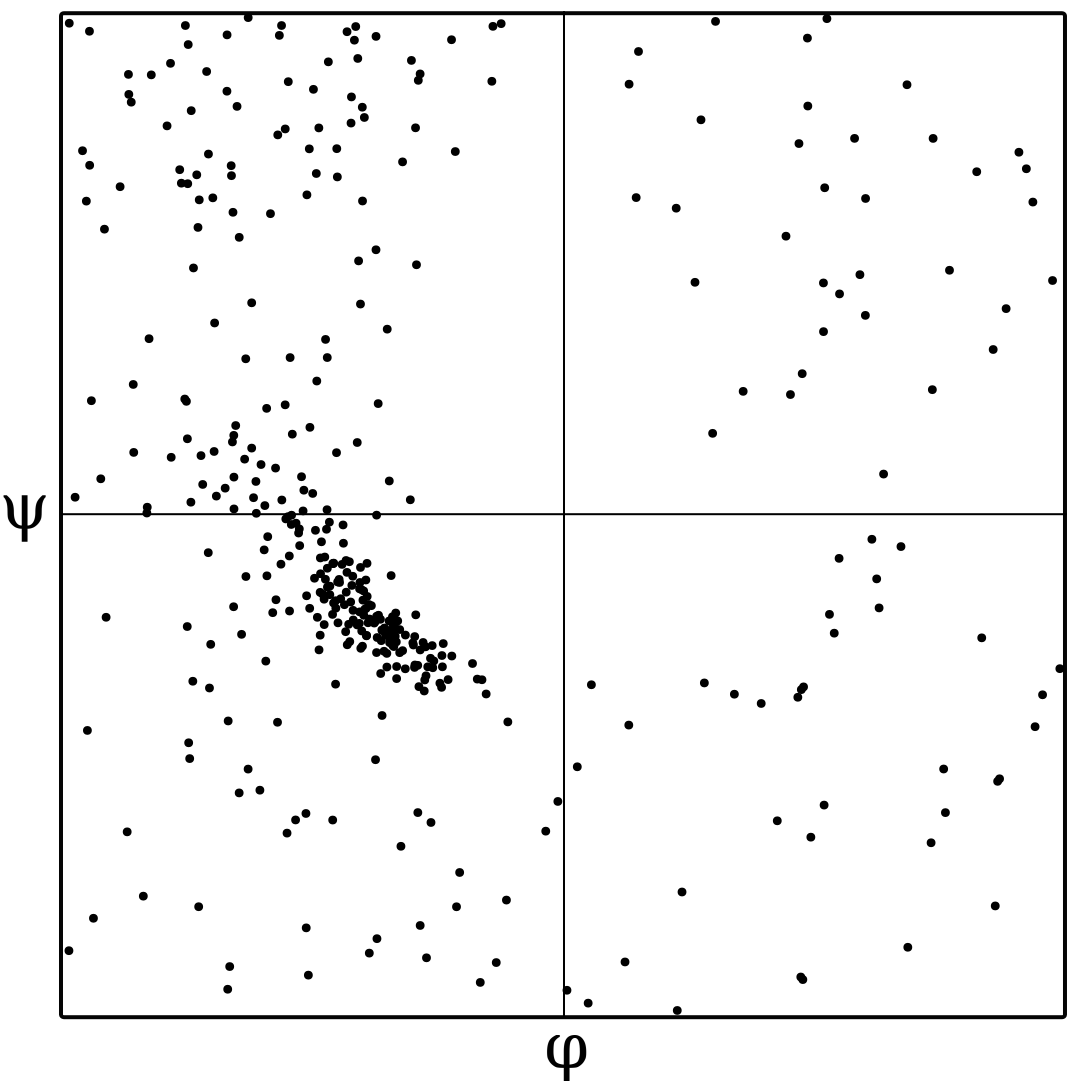
\includegraphics[width=0.75\columnwidth]{figures/plot_ramachandran}\hspace{1cm} }
	\caption{Ramachandran plot of \textbf{(a)} an original protein of length 415 \textbf{(b)} a protein backbone fitted to the original protein (RMSD $=0.15$ Å).}
	\label{fig:eval_ramachandran}
\end{figure*}


\section{Collision handling}
With the backbone in place the side-chain rotamers are chosen such that the number of collisions is minimized.
There is a correlation between the average number of collisions in a fitted protein and how well we are able to fit it to the backbone. 
For small RMSDs, the number of collisions is around 1 per 75 amino acids.
	%Thus, collisions are more likely to occur in large proteins.

In Figure \ref{fig:plot_scp} we have plotted the average number of collisions after SCP as a function of the number of initial collisions.
In our experience, the collision avoidance algorithm is working quite efficiently reducing the number of collisions in a protein from 10 to 1 on average.
We have performed a visual inspection on the remaining collisions and the majority of the collisions is caused by either: 
1. A proline amino acid is given an unfavorable set of $\phi$ and $\psi$ angles such that the backbone will collide with all of the proline rotamers.
2. The backbone is folded unfavorably such that the amino acids too close making side-chain collisions inevitable
Thus, both problems are caused by a deficient fitting algorithm.

Varying the search depth parameter for the SCP algorithm has little effect for depths over 3.
When the search depth is below 3 we see that the number of resolved collisions drops.

\label{sec:evaluation_handling_side-chains}
\begin{figure}
	\centering
	\hspace*{-3.5mm}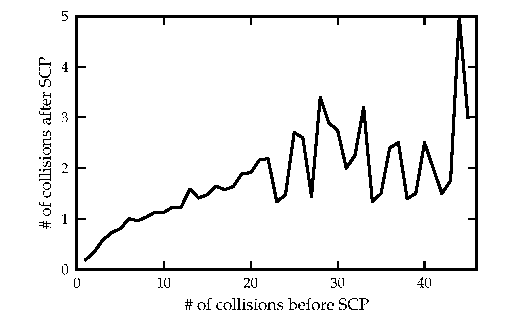
\includegraphics[width=1.1\columnwidth]{figures/plot_scp}
	\caption{SCP performance: The average number of collisions as a function of the number of initial collision. The fluctuations in the right half of the plot is caused by noise.}
	\label{fig:plot_scp}
\end{figure}

